\documentclass[border=10pt]{standalone}

\usepackage{tikz}
\usepackage{tikzsymbols}
\usetikzlibrary{calc,patterns,shapes.geometric}

\def\centerarc[#1](#2)(#3:#4:#5){\draw[#1] ($(#2)+({#5*cos(#3)},{#5*sin(#3)})$) arc (#3:#4:#5);}

\begin{document}
	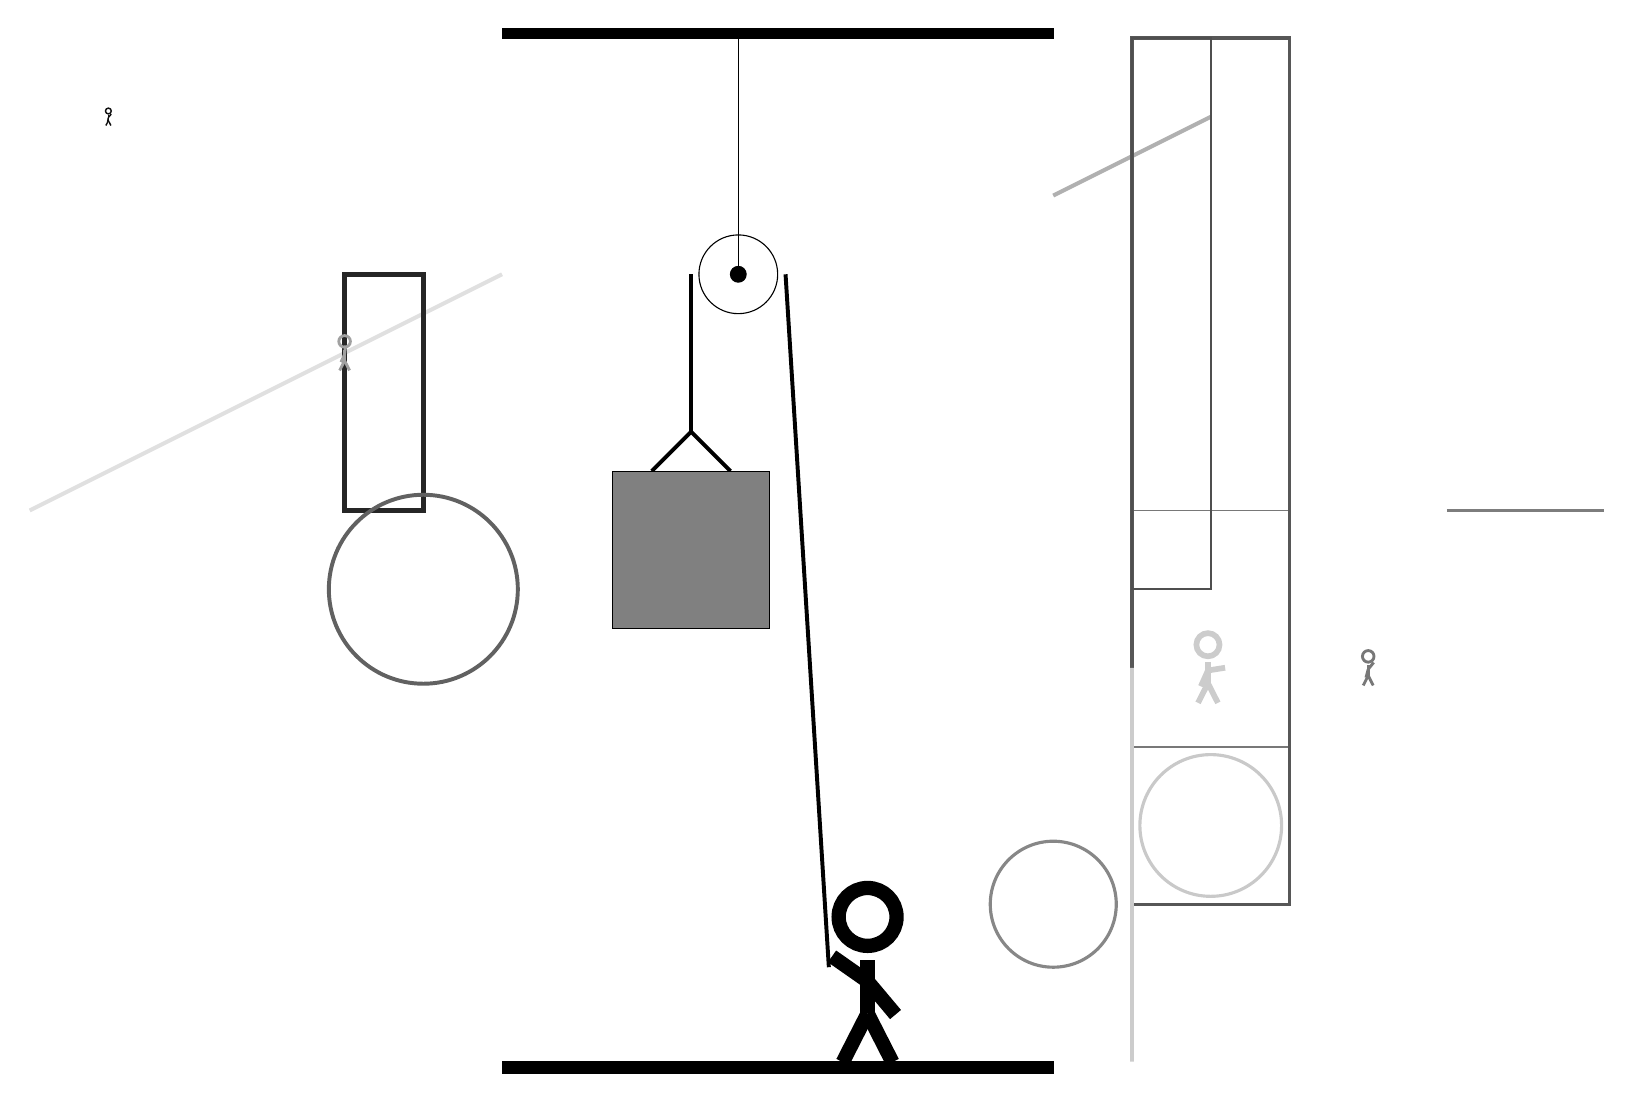
\begin{tikzpicture}
		%%%%% START %%%%%
		
		\draw[fill=black] (-2, 10) rectangle (5, 10.125);
		
		\draw [line width=0.4mm, color=black!21](7, 0) circle (0.9);
		
		\draw[line width=0.5mm, color=black!51](10, 4) -- (12, 4);
		\node[line width=0.4mm, color=black!20] at (7, 2) {\Strichmaxerl[4][66][9]};
		\draw[line width=0.5mm, color=black!12](-2, 7) -- (-8, 4);
		
		\draw [line width=0.4mm, color=black!47](5, -1) circle (0.8);
		\node[line width=0.4mm, color=black!53] at (9, 2) {\Strichmaxerl[2][75][51]};
		
		\draw[line width=0.5mm, color=black!31](5, 8) -- (7, 9);
		
		\draw[line width=0.7mm, color=black!85] (-4, 4) rectangle (-3, 7);
		\draw[line width=0.2mm, color=black!53] (6, 4) rectangle (8, 1);
		\draw[line width=0.4mm, color=black!66] (6, 10) rectangle (8, -1);
		\draw [line width=0.5mm, color=black!62](-3, 3) circle (1.2);
		\draw[line width=0.6mm, color=black!20] (6, -3) rectangle (6, 2);
		\node[line width=0.6mm, color=black!94] at (-7, 9) {\Strichmaxerl[1][79][49]};
		
		\draw[line width=0.3mm, color=black!69] (6, 3) rectangle (7, 10);
		\node[line width=0.2mm, color=black!37] at (-4, 6) {\Strichmaxerl[2][65][83]};
		
		\draw (1, 7) circle (0.5);
		\draw[fill=black] (1, 7) circle (0.1);
		\draw (1, 10) -- (1, 7);
		
		\draw[line width=0.5mm] (-0.1, 4.5) -- (0.4, 5.0) -- (0.9, 4.5);
		\draw[fill=black!50] (-0.6, 4.5) rectangle (1.4, 2.5);
		
		\draw[line width=0.5mm] (0.4, 7) -- (0.4, 5.0);
		\centerarc[line width=0.5mm](1, 7)(0:180:0.6);
		\draw[line width=0.5mm](1.6, 7) -- (2.15, -1.8);
		
		\node at (2.6, -1.9) {\Strichmaxerl[10][-35][-50]};
		
		\draw[fill=black] (-2, -3) rectangle (5, -3.15);
		
		%%%%% END %%%%%
	\end{tikzpicture}
\end{document}